% 
% Annual Cognitive Science Conference
% Sample LaTeX Paper -- Proceedings Format
% 

% Original : Ashwin Ram (ashwin@cc.gatech.edu)       04/01/1994
% Modified : Johanna Moore (jmoore@cs.pitt.edu)      03/17/1995
% Modified : David Noelle (noelle@ucsd.edu)          03/15/1996
% Modified : Pat Langley (langley@cs.stanford.edu)   01/26/1997
% Latex2e corrections by Ramin Charles Nakisa        01/28/1997 
% Modified : Tina Eliassi-Rad (eliassi@cs.wisc.edu)  01/31/1998
% Modified : Trisha Yannuzzi (trisha@ircs.upenn.edu) 12/28/1999 (in process)
% Modified : Mary Ellen Foster (M.E.Foster@ed.ac.uk) 12/11/2000
% Modified : Ken Forbus                              01/23/2004
% Modified : Eli M. Silk (esilk@pitt.edu)            05/24/2005
% Modified : Niels Taatgen (taatgen@cmu.edu)         10/24/2006
% Modified : David Noelle (dnoelle@ucmerced.edu)     11/19/2014
% Modified : Roger Levy (rplevy@mit.edu)     12/31/2018



%% Change "letterpaper" in the following line to "a4paper" if you must.

\documentclass[10pt,letterpaper]{article}
\usepackage{cogsci}
%\usepackage{dsfont}
\usepackage{bm}
\usepackage{amssymb}
\usepackage{indentfirst}
\usepackage{graphicx}
\usepackage{subfig}
\usepackage{multirow}

%\cogscifinalcopy % Uncomment this line for the final submission 


\usepackage{pslatex}
\usepackage{apacite}
\usepackage{float} % Roger Levy added this and changed figure/table
                   % placement to [H] for conformity to Word template,
                   % though floating tables and figures to top is
                   % still generally recommended!

\newcommand{\ev}[2]{$#1_#2$}

%\usepackage[none]{hyphenat} % Sometimes it can be useful to turn off
%hyphenation for purposes such as spell checking of the resulting
%PDF.  Uncomment this block to turn off hyphenation.


%\setlength\titlebox{4.5cm}
% You can expand the titlebox if you need extra space
% to show all the authors. Please do not make the titlebox
% smaller than 4.5cm (the original size).
%%If you do, we reserve the right to require you to change it back in
%%the camera-ready version, which could interfere with the timely
%%appearance of your paper in the Proceedings.



%\title{A continuity-based account of actual causation}
%\title{Identifying actual causes by tracking Changes of State in Continuous Time}
\title{Actual Causes as Changes of State in Continuous Time}
 
\author{{\large \bf Morton Ann Gernsbacher (MAG@Macc.Wisc.Edu)} \\
  Department of Psychology, 1202 W. Johnson Street \\
  Madison, WI 53706 USA
  \AND {\large \bf Sharon J.~Derry (SDJ@Macc.Wisc.Edu)} \\
  Department of Educational Psychology, 1025 W. Johnson Street \\
  Madison, WI 53706 USA}


\begin{document}

\maketitle


\begin{abstract}

\textbf{Keywords:} 
\end{abstract}


\section{Introduction}


Around 5:27 pm on November 9, 1965, Martin Saltzman found himself trapped in a dark elevator roughly a quarter of a way up the Empire State building~\cite{rosenthalg65}. The stopping of Saltzman's elevator was one of thousands of unexpected events that occurred that evening, and virtually all of the people involved must have wondered about the causes of these events. Subsequent accounts of the Great Northeastern Blackout often trace these events back to the tripping of a relay on line Q29BD in Ontario that triggered a cascade of failures.

Identifying the cause of an event (e.g.\ the stopping of an elevator) requires a judgment of actual causation, also known as singular or token causation~\cite{danks17}. Psychologists and philosophers have explored these judgments in detail~and developed formal models of actual causation, including models based on Bayesian networks \cite{}, force dynamics \cite{wolff} and physical simulation~\cite{gerstenberg}.  Here we present and evaluate an account of actual causation that highlights the role of temporal continuity.  On this account, the tripping of relay Q29BD is the main cause of the elevator stopping because the tripping initiated a continuous sequence of state changes that culminated in the stopping of the elevator.

Most accounts of actual causation are consistent with one of two broad views of causation: the counterfactual approach and the physical process approach. The counterfactual approach suggests that the tripping of relay Q29BD is a cause of the elevator stopping because if the relay had not tripped then the elevator would not have stopped. The physical process view suggests that the relay tripping is a cause of the elevator stopping because the two are linked by a physical process involving the transmission of force or energy.  Both accounts need additional machinery in order to specify which among the many causes of an event is singled out as the main cause. Our continuity account fits most naturally with the physical process approach, and can be viewed as an attempt to bring out some implications of this approach for actual causation. 

Two key principles. 

Limited in scope.




Like most other formulations of the physical process view, our






Identifying the causes of an event involves not only logical rules but also different senses of ``causation'' that people might have. Let's imagine that, to mitigate false alarms rate and improve the detection of fires, Lilly decides to install at home a dual alarm system that goes off if and only if two chains of ionization and photoelectric detectors are triggered (Fig.\ref{fig:1}a). Lilly wants to test her new system by exposing the detectors to some smoke. At some point a ionization detector starts beeping first while measuring a change in the electrical conductivity of air. It activates the next detector in the sequence which then activates the last one (Fig.\ref{fig:1}b). At this stage Lilly notices that the alarm remains silent. After a while a photoelectric detector starts beeping as well while measuring a change in the transparency of air. It activates the next detector in the sequence which then activates the last one and right after the alarm goes off (Fig.\ref{fig:1}c). 

\begin{figure*}
\begin{center}
%\includegraphics[width=7cm]{figures/demo.eps}
\includegraphics{figures/introfig.eps}
\end{center}
\caption{(a)(i) A smoke alarm connected to a chain of ionization detectors (top branch) and a chain of photoelectric detectors (bottom branch). All components are initially inactive (ii) Detector \ev{R}{D} activates and activity propagates along the top branch. (iii) Detector \ev{R}{C} activates and ultimately triggers the activation of the alarm, which activates only when both  \ev{I}{D} and \ev{I}{C} are active. (b) An activation sequence in which (i) the top branch activates first, (ii) activation starts and finishes along the bottom branch while activation continues along the top branch, and (iii) the top branch completes its activation and ultimately triggers the smoke alarm.}
\label{fig:intro}
\end{figure*}

What would Lilly think caused the alarm to go off? Several answers can be considered. Based on logical dependencies, people's causal judgements can state that both the furthest activated ionization detector (first root change ``R1'') and the furthest activated photoelectric detector (second root change ``R2'') are equally the causes of the alarm activation. However a more intuitive answer would be that the provided temporal information influences people's choice toward one cause more than the other one. An important selection criterium could be how recent a candidate cause is compared to another one and would lead for instance to the following preferences: R2 $\succ$ R1, and I2 $\succ$ I1 (``I2'' and ``I1'' being respectively the second and first immediate changes). Nonetheless we can imagine other cases where people potentially rely in part on another type of temporal criterium: let's imagine that the activation of the ionization detectors starts before and finishes after the activation of the photoelectric detectors, such that R1 and I2 are linked by a \textit{continuous sequence of changes}. In that case this is the activation of the oldest root change R1 and not the most recent root change R2 that initiate a continuous sequence of changes until the activation of the alarm. In such situations we want to know what people would consider as the main cause of the system.

The alarm case can be seen as an example of ``singular causation''\footnote{Also called ``token'' or ``actual causation'' by opposition with ``general causation'' -- following a distinction that has been frequently made in the litterature.} where we want to understand, in a singular context, what caused a particular event to occurr at the time it did. Here specifically it instantiates a class of causal systems where an event is a common effect of distinct sequences of necessary causes. Causal judgements have been widely studied in the litterature, however the temporal order in which each variable changes its value is an important feature of causal systems that have been hardly studied nor tested experimentally as we intended to do. Indeed current research on actual causation mainly relies on two different interpretations of causality that don't ground causal judgements on temporal information: the counterfactual (CF) and the physical process (PP) accounts. On the one hand, in the CF framework, events are represented as mere propostions and causation is thought as a relation between static states (A is a cause of B if and only if A and B are true, and A hadn't occurred B wouldn't have occurred). On the other hand the PP account is meant to give an epistemological definition of the concept of causation and not an explanation of how people actually rely on temporal informations to make causal judgements.

In this paper we present two experiments that show the importance of taking into account temporal information to explain the causal judgements people make. In particular we relied on the intuition behind the example above that the chronological order and the temporal relationship between distinct causes can bias people toward an event rather than another in considering which one is the main cause of the effect.

% Intro:
% smoke detector example
% 

\section{The continuity account of actual causation}

This section uses the smoke detector example in Figure~\ref{fig:intro}a to introduce our theoretical approach to actual causation. Like physical process theory, we focus on processes unfolding in continuous time, but it will be convenient to divide up the temporal dimension into intervals brief enough that there is at most one event per interval. The effect to be explained is an event that happens within one of these intervals: for example, a smoke alarm's change of state from inactive to active. Given this setup, our theory can be formulated using a procedure that starts with the effect and steps backwards through time until the actual cause of the effect is identified.

The immediate cause of the smoke alarm's activation must be an event that took place in the interval preceding the activation. In Figure~\ref{fig:intro}a, the event immediately preceding the alarm's activation was the activation of \ev{I}{C}. Having identified this immediate cause, we then step backwards and identify the immediate cause of this event, and so on.  The procedure terminates once we arrive at an event that has no immediate cause within the system of interest, 
and this cause is declared to be the main cause of the effect.  In Figure~\ref{fig:intro}a the main cause is the activation of \ev{R}{C}. 

In most cases, the backward-tracing procedure just described will identify a single main cause of the effect. If the effect has no immediate cause within the system, then no main cause will be identified. Because there is at most one event per interval, the procedure can never identify more than one main cause.

The assumption that at most one event occurs per interval follows from the idea that there are no coincidences. In continuous time it is exceedingly improbable that two events would occur at exactly the same time --- in technical terms this kind of coincidence can be described as a ``measure zero'' possibility. If there are no coincidences, then slicing the time dimension sufficiently finely will ensure that there is at most one event per interval.

The boundaries of the causal system under consideration will depend on context. For simplicity, our discussion of Figure~\ref{fig:intro}a focused only on events internal to the alarm system, and addressed the question of which detector is best viewed as the main cause of the alarm's activation. Questions about smoke alarms, however, will often be framed with respect to a causal system that includes both the alarm system and its surroundings. Expanding the causal system in this way may allow the alarm's activation to be traced back to an event such as an electrical fault that started a fire that generated smoke that triggered the alarm.



%So far it seems that none of the current main theories of actual causation has focused on the role of temporal information for inferring causal relationship between events qua changes of states over time. In contrast we hypothesised that people's causal judgements are influenced not only by the values of all relevant variables at the time the effect occurs, but also the temporal order in which these variables took their values. This approach has some precedent in the literature but has not been developed carefully and has never been tested experimentally as we intend to do. We add further that people mainly identify causation with a \textit{continuous} sequence of changes of states over time. The underlying intuition is that people trace back the history of changes from the immediate one that directly brought about the occurrence of the effect, up to the root change in the system that initiated the series of changes along the path. As we think that in common life it is really rare to see simultaneously two or more events occurring at the very same time and producing some common effect, we also want to postulate a \textit{no coincidence principle}. Relying on this principle we can split the system's time frame in units of time that are small enough to have no more than one event\footnote{Again we insist on the definition of \textit{event} as \textit{change of state}.} per unit. Lets represent by $\mu^{\emptyset}_{z_{i\rightarrow j}}(t)$ a change of state at time $t$, from variable $Z=z_i$ to $Z=z_j$, $\forall i,j\in {R}_+$. Here $Z$ is the variable we want to reason about and has no children (represented by the empty set $\{\emptyset\}$). Formalizing our above mentioned idea we first have to find $\mathcal{U}^Z_{\bm{y}_{i\rightarrow j}}(t-1)$, that is the set of the immediate changes in the parents $\bm{Y}$ of the variable $Z$ at time $t-1$ that led to the observed change in $Z$ at time $t$. So we want to find $\mathcal{U}$ such that $\mathcal{U}^Z_{\bm{y}_{i\rightarrow j}}(t-1)\rightarrow \mu^{\emptyset}_{z_{i\rightarrow j}}(t)$. According to our \textit{no coincidence principle} $\mathcal{U}$ is either empty or a singleton -- including only one parent whose value changed. Lets say that at $t-1$ we find a change in a parent variable $Y$, so $\mathcal{U}^Z_{\bm{y}_{i\rightarrow j}}(t-1)=\{\mu^{Z}_{y_{i\rightarrow j}}(t-1)\}$. Then we want to find the set of changes such that $\mathcal{U}^Y_{\bm{x}_{i\rightarrow j}}(t-2)\rightarrow \mu^{Z}_{y_{i\rightarrow j}}(t-1)$, that is the set of immediate previous changes in the parents $\bm{X}$ of the variable $Y$ at time $t-2$ that led to the observed change in $Y$ at time $t-1$. Following the same logic we suggest that if $\mathcal{U}^X_{\bm{w}_{i\rightarrow j}}(t-3)\rightarrow \mu^{Y}_{x_{i\rightarrow j}}(t-2)$ is such that $\mathcal{U}^X_{\bm{w}_{i\rightarrow j}}(t-3)=\emptyset$, then it means that $\mu^{Y}_{x_{i\rightarrow j}}(t-2)$ represents the chronologically first change along the path, occurring in $X$, and we suggest that this change is identified as being the main cause of $Z$.

\section{Experiments}

We developed two experiments to test the continuity account of actual causation just presented.  
%The first experiment explores some simple cases directly analogous to the smoke detector example. The second experiment explores cases that elaborate that distinguish between the continuity account and Spellman's probability raising account~\cite{spellman97}.
The cover story asked participants to imagine that they worked in a nuclear control room and that their job was to monitor networks of particle detectors. Detectors were shown as white squares (as in Figure~\ref{fig:intro}) that become active and turn black when they absorb a radioactive particle. Activation is transmitted across links in the network, and a detector activates if all of its input detectors are active. Each network contains a special detector called the Gauge of Critical Moment (GCM, analogous to the smoke alarm in Figure~\ref{fig:intro}a) and participants were told that ``for each activation sequence that you see, your job is to decide what caused the activation of the GCM.'' 

Both experiments included chains in which the GCM received input from one detector, and dual branch networks such as Figure~\ref{fig:intro}a in which the GCM received input from two detectors. For chains, the continuity account predicts that participants will tend to choose the root cause of the effect (ie the detector that initiates the activation sequence) rather than the immediate cause (the detector that immediately precedes the GCM). For dual branch networks, the continuity account predicts that participants will tend to choose the root cause on the branch whose activation is temporally continuous with the activation of the GCM. We refer to this branch as the continuous branch, and refer to the root cause and the immediate cause on this branch as \ev{R}{C} and \ev{I}{C} respectively, where the subscript denotes ``continuous.'' We refer to the other branch as the ``delayed branch,'' and use \ev{R}{D} and \ev{I}{D} for the root and immediate causes on this branch. The ``delay'' in this naming scheme refers to the delay that occurs between \ev{I}{D} and the activation of the GCM. It is convenient to use the same labels for both detectors and events: for example, \ev{R}{C} will be used to denote both a detector on the continuous branch and the activation of this detector. This flexible use of notation, however, does not imply that actual causation involves a relationship between objects rather than events.

Our presentation of the experiments focuses on two theoretical accounts: the continuity account and the probability raising account. For completeness, though, we first discuss the counterfactual and physical process accounts. Both accounts can be formulated in different ways. Here we present what we take to be the default predictions of the two accounts, and the General Discussion considers ways in which the accounts can be adjusted to make different predictions. 

The counterfactual account makes no clear prediction about whether root causes or immediate causes should take priority. For a chain network, if the root cause had not occurred, the effect would not have occurred, but if the immediate cause had not occurred, the effect would also not have occurred. If we consider dual branch networks and restrict attention to root causes only, then the account makes no clear prediction about whether \ev{R}{C} should be preferred to \ev{R}{D}.  If \ev{R}{C} had not occurred, then the effect would not have occurred, and likewise for \ev{R}{D}.  

The physical process account is similarly inconclusive. Both root and immediate causes are connected by a physical process to the effect, and there seems to be no clear reason for preferring one to the another. If we focus only on root causes, again there is no clear preference between \ev{R}{C} and \ev{R}{D}. After the activation of \ev{I}{D}, one can think of this detector as continuously sending activation towards the GCM which only ``unlocks`` the detector once \ev{I}{C} is also active. It follows that both \ev{R}{C} and \ev{R}{D} are connected to the effect by physical processes.

Because both of these accounts make no clear predictions, it seemed possible that people's inferences about the networks in our experiments would be highly variable and would reveal no clear trends. Our first experiment therefore explored simple cases analogous to the smoke detector example in Figure~\ref{fig:intro} with the goal of establishing whether the basic experimental procedure was viable.  The second experiment focused on more elaborate dual-branch cases that aimed to distinguish between the continuity account and Spellman's probability raising account~\cite{spellman97}.

\subsection{Experiment 1}

Experiment 1 included both causal chains and dual branch networks. For all of the dual branch stimuli, \ev{I}{D} occurred before \ev{R}{C} (Figure~\ref{fig:expt1}a) which means that the delayed branch completed its activation before the continuous branch began to activate. The probability raising and continuity accounts both predict that root causes should be preferred to immediate causes, and that for dual branch networks \ev{R}{C} should be preferred to \ev{R}{D}. The primary purpose of the experiment was to test both predictions. 

\textbf{Participants}. 30 participants were recruited via Amazon Mechanical Turk and paid XXX for a YYY minute experiment.

%The experiment was hosted by Google Cloud App Engine and 30 participants were recruited via Amazon Mahchanical Turk. There were 10 females (average age: 37.3) and 20 males (average age: 37.6). 28 participants were english speakers, 1 were italian speaker and 1 marathi speaker.


\textbf{Materials}. The experiment used a customized interface built using the jsPsych library~\cite{XXX}. For all networks presented, participants clicked a ``Run'' button to observe an activation sequence. The first event in the sequence (i.e.\ the first change of state) always took place 5 seconds after the Run button was clicked, and the delay between successive activations along a chain of detectors was set to 100 ms. After the final event in a sequence (i.e.\ the activation of the GCM), all detectors became clickable after a delay of 1 second. Clicking on a detector turned its border red, and at most one detector could be selected at any time. After a sequence completed, participants could view it again if they wished by clicking a ``Run again'' button.

\textbf{Design}.  The experiment included activation sequences over 15 networks (3 chains and 12 dual branch networks). Excluding the GCM, each chain and each branch of each dual network had 7 detectors. We refer to the sequences as \emph{short}, \emph{medium} or \emph{long} based on the distance between the root causes and the GCM. Excluding the GCM, the short, medium and long chain sequences showed 1, 3 and 6 active detectors respectively at the end of the sequence. Within each dual branch sequence, the root causes on the two branches (\ev{R}{D} and \ev{R}{C}) were equidistant from the GCM, but these distances varied across sequences. The sequence in Figure~\ref{fig:intro}a is a medium dual branch sequence (3 active detectors in each branch excluding the GCM), and short and long versions had 1 and 6 active detectors respectively per branch.

Each dual branch sequence (short, medium and long) came in four versions. The \emph{state} version showed the delayed branch (including detectors \ev{R}{D} and \ev{I}{D}) as active from the very beginning of the sequence. The activation of this branch was therefore presented as having occurred at some indefinite time in the past, resulting in a steady state of activation. The three \emph{event} versions all showed \ev{R}{D} activating 5 seconds into the sequence, and had delays of 2, 4 and 6 seconds between the activation of \ev{I}{D} and \ev{R}{C}.


\textbf{Procedure}. 
Participants first read instructions which introduced the task and included examples of a chain and a dual branch network. They then answered three questions about the task and the detectors, and were sent back to read the instructions again if they answered incorrectly. They continued cycling through the instructions and the test questions until they answered all questions correctly.

The 15 activation sequences in the experiment proper were presented in random order. For dual branch sequences, the vertical position of the delayed branch was also randomized (Figure~\ref{fig:intro} shows the delayed branch on the top rather than the bottom). The orientation of the network (GCM on the left or the right) was randomized within participants.  The prompt after each sequence was ``In this sequence what caused the activation of the GCM? Respond by clicking on a detector,'' and participants were required to choose a single detector in response. 

\textbf{Results}. 
Network orientation (left or right) and position of the delay branch (top or bottom) had no apparent effect, and we therefore collapse across these variables. Figure~\ref{fig:expt1} summarizes the results for short, medium and long dual-branch sequences. The delay between \ev{I}{D} and \ev{R}{C} had no significant effect, and Figure~\ref{fig:expt1} combines results for all three delays.  

Although \ev{R}{D}, \ev{I}{D}, \ev{R}{C} and \ev{I}{C} all qualify as causes of the effect, Figure~\ref{fig:expt1} suggests that \ev{R}{C} tends to be singled out as the main cause. This result can be separated into two general conclusions.  First,  participants were more likely to choose root causes than immediate causes. Root and immediate causes were identical for the short sequences and therefore cannot bet distinguished, but the results for medium and long sequences reveal a preference for root causes. STATISTICAL ANALYSIS. 

The second conclusion is that for dual branch sequences, the root cause on the continuous branch (\ev{R}{C}) is preferred to the root cause on the delayed branch (\ev{R}{D}). This result is consistent with the continuity account but also consistent with the probability raising account, because \ev{R}{C} guarantees the occurrence of the effect but \ev{R}{D} does not. 

Figure \ref{fig:intro} suggests that event and state sequences lead to similar patterns of responses. The continuity account makes the same prediction for both kinds of sequences, but we anticipated that the event sequences might make participants especially likely to choose \ev{R}{C} over \ev{R}{D}. If this effect exists, our data suggest that it is relatively small.

It is notable that people's judgments are largely unaffected by the delay between \ev{I}{D} and \ev{R}{C} and the activation length of each sequence (short, medium or long). Both of these variables affect the time that elapses between the root causes and the effect, and our results suggest that people's judgments are not exquisitely sensitive to this sort of variation.

Thus far we have focused on dual branch sequences, and the chain sequences are of interest primarily because they provide additional evidence of a preference for root causes.  NUMBERS HERE



%First of all we observed no significant effect [STATISTICS?] of neither the orientation of the networks (left \textit{vs} right) nor the location where the activation starts first (top \textit{vs} bottom). On average participants took 14 min to complete the experiment and overall 96\% of the time participants run an animation only once. Second of all the results show two main findings: first the length of the activation sequences (one, three or six detectors in each branch of the AND-Gates) has no effect on the response pattern; second neither the delay between I1 and R2 (2000ms, 4000ms and 6000ms) nor the fact that some detectors were already activated in State condition have a significant effect on causal judgement. So overall people massively chose the last root change R2 as the main cause of the GCM activation for medium and long networks (and R2/I2 for the short networks since both were identical). For the short networks (state and event types combined) 25\% \textit{vs} 65\% of participants chose respectively R1/I1 \textit{vs} R2/I2 as the main cause; for the medium networks (state and event combined) we got 23\% \textit{vs} 53\% for respectively R1 and R2 and 20\% \textit{vs} 55\% for the long networks (Fig.\ref{fig:2}). 

%[WARNING: THE GRAPH BELOW SHOW THE RESULTS FOR SHORT, MEDIUM, LONG \textbf{LENGTHS} (ALL THE DELAYS MIXED) SO NOT THE DIFFERENT DELAYS BETWEEN I1 AND R2. BUT AS OUR FOCUS IS ON TEMPORAL INFORMATION, MAYBE WE SHOULD GRAPHICALLY SHOW THAT THE DELAY HAS NO EFFECT?? BUT IT MEANS THAT WE HAVE TO ADD TWO MORE COLUMNS FOR EACH DETECTOR CATEGORY]

\begin{figure}
\begin{center}
%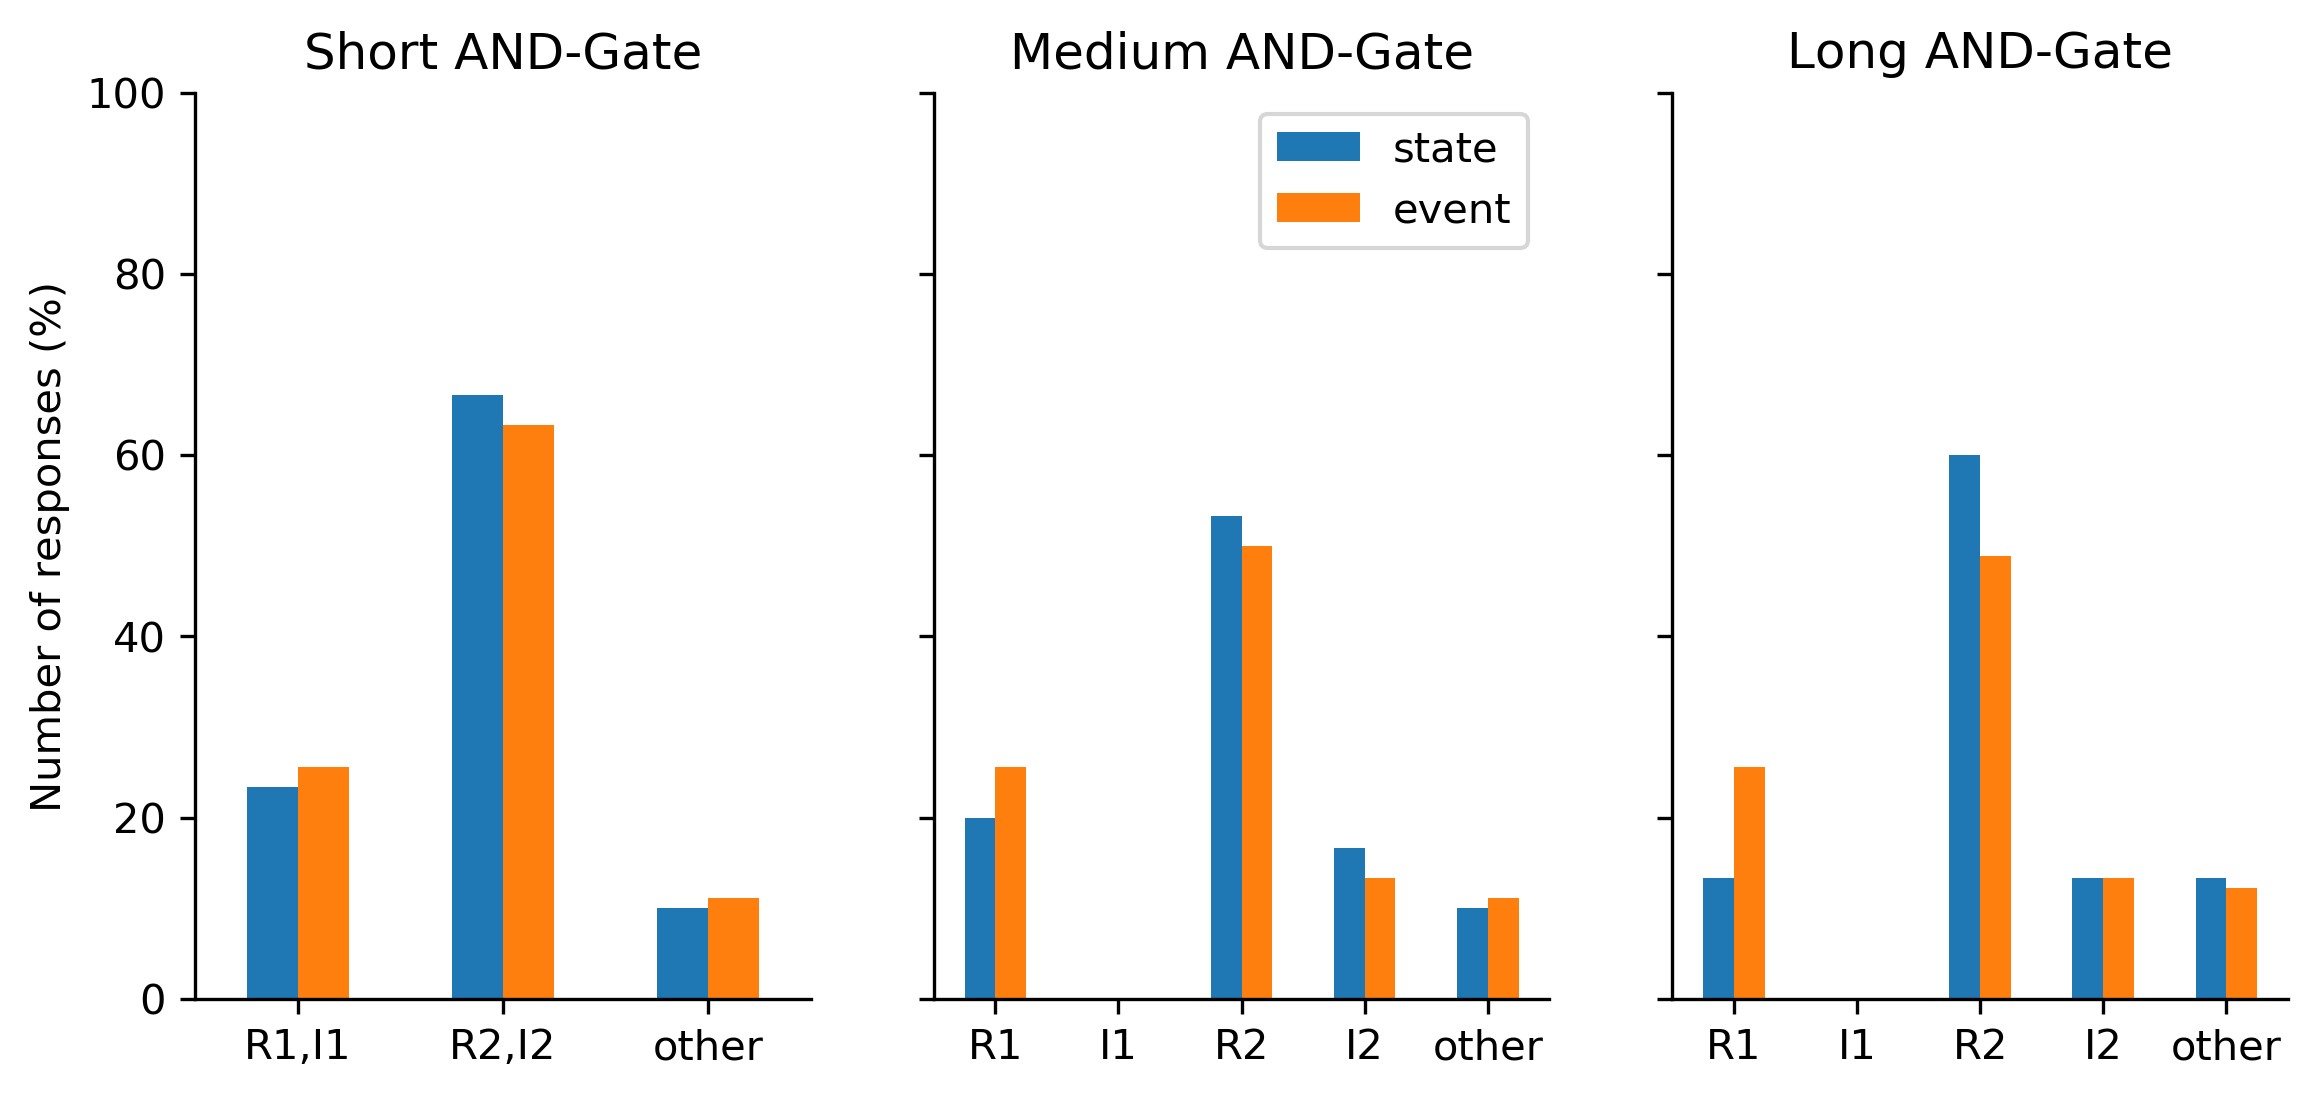
\includegraphics[width=8cm]{results_E1}
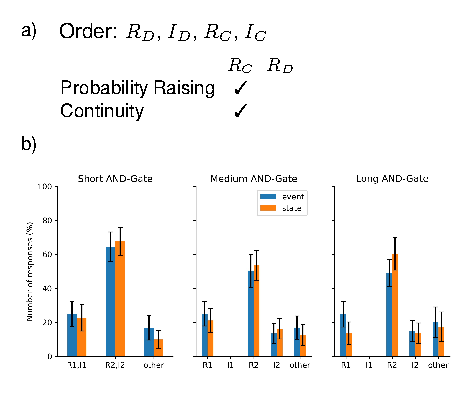
\includegraphics{figures/expt1.eps}
\end{center}
\caption{Experiment 1. (a) Order of the four key events for dual branch sequences. The probability raising and continuity accounts both single out \ev{R}{C} as the main cause. (b)  Responses for dual branch sequences. The delayed branch was either inactive (event sequences) or active (state sequences) at the start of the sequence.} 
\label{fig:expt1}
\end{figure}

\subsection{Experiment 2}

The results of Experiment 1 are broadly consistent with both the continuity and probability raising accounts, and the goal of Experiment 2 was to distinguish between these accounts. The two make different predictions for dual branch sequences in which the delayed branch activates after activation has already begun along the continuous branch. One such sequence is shown in Figure~\ref{fig:intro}b. 
In cases like this, \ev{R}{D} guarantees the occurrence of the effect, and therefore qualifies as the primary cause according to the probability raising account. The continuity account, however, still treats \ev{R}{C} as the primary cause.

The materials and procedure for Experiment 2 are similar to those for Experiment 1, and we highlight only the few points of difference.

\textbf{Participants}. 100 participants were recruited via Amazon Mechanical Turk and paid XXX for a YYY minute experiment. Two did not submit a valid completion code, leaving 98 sets of responses for analysis.

%The experiment was hosted by Google App Engine and 98 participants were recruited via Amazon Mechanical Turk. There were 40 females (average age: 40.4), 57 males (average age: 37.6) and 1 declared ``other''. All the participants were english speakers except for 2 participants.

\textbf{Design}. 
The experiment included one chain sequence and 6 dual branch sequences. Each dual branch included one straight branch and a longer curved branch, as shown in Figure~\ref{fig:intro}b. The dual branch sequences included the events \ev{R}{C}, \ev{R}{D}, \ev{I}{C}, and \ev{I}{D} in three different orders shown in Figures~\ref{fig:expt2}a and \ref{fig:expt2}b. The sequence in Figure~\ref{fig:intro}b is an instance of the order in Figure~\ref{fig:expt2}a, because the activation on the delayed branch starts (\ev{R}{D}) and finishes (\ev{I}{D}) while activation is propagating along the continuous branch. The 6 dual branch sequences included 2 variants of each of the three orders. In one variant \ev{R}{C} belonged to the curved branch (as in Figure~\ref{fig:intro}b) and in the other \ev{R}{C} belonged to the straight branch. 

% XXX: event vs state?


\textbf{Procedure}. 
The position of the curved branch (top or bottom) was randomized. The presentation order of the activation sequences and the orientation (GCM on the left or right) were randomized as for Experiment 1.
%In Experiment 2 each participant was presented 7 different networks. One stimulus was a chain and all the other six stimuli were AND-Gates. Like in Experiment 1 we tested for the dimension ``Event'' \textit{vs} ``State''. Same as before in condition ``Event'' none of the detectors was initially active and in condition ``State'' one of the two branches was containing detectors that were already active before the animation started. However this time, within the condition ``Event'',  we also tested for the extra dimension ``R1 cont'' \textit{vs} ``R2 cont''.  In condition ``R1 cont'' (represented in Fig.\ref{fig:3}) the activation is such that there is a continuous sequence of changes going from R1 to I2 leading to the activation of G. In condition ``R2 cont'' (not represented here) this is R2 that was continously connected to I2 leading to the activation of G. For the AND-Gates the delay between I1 and I2 in condition ``Event'' was maintained at 11 nodes (i.e.1100 ms) for almost all the networks. There was only one network for which the delay was set at 8 nodes (800ms).

%As in Experiment 1 participants were first presented the network in its initial state and were asked to click the ``Run'' button to observe an activation sequence over the network. Participants waited 5000ms to see a first change of state occurring in a detector. Activation delay between any two successive square activations was set on 100ms as well. All the stimuli were presented in a random order and participants were assigned to either group "Left" or "Right" as in Experiment 1, and each AND-Gate was randomly presented with the curved chain (see Fig.\ref{fig:3})) at the top or at the bottom.

%\begin{figure}[ht]
%\begin{center}
%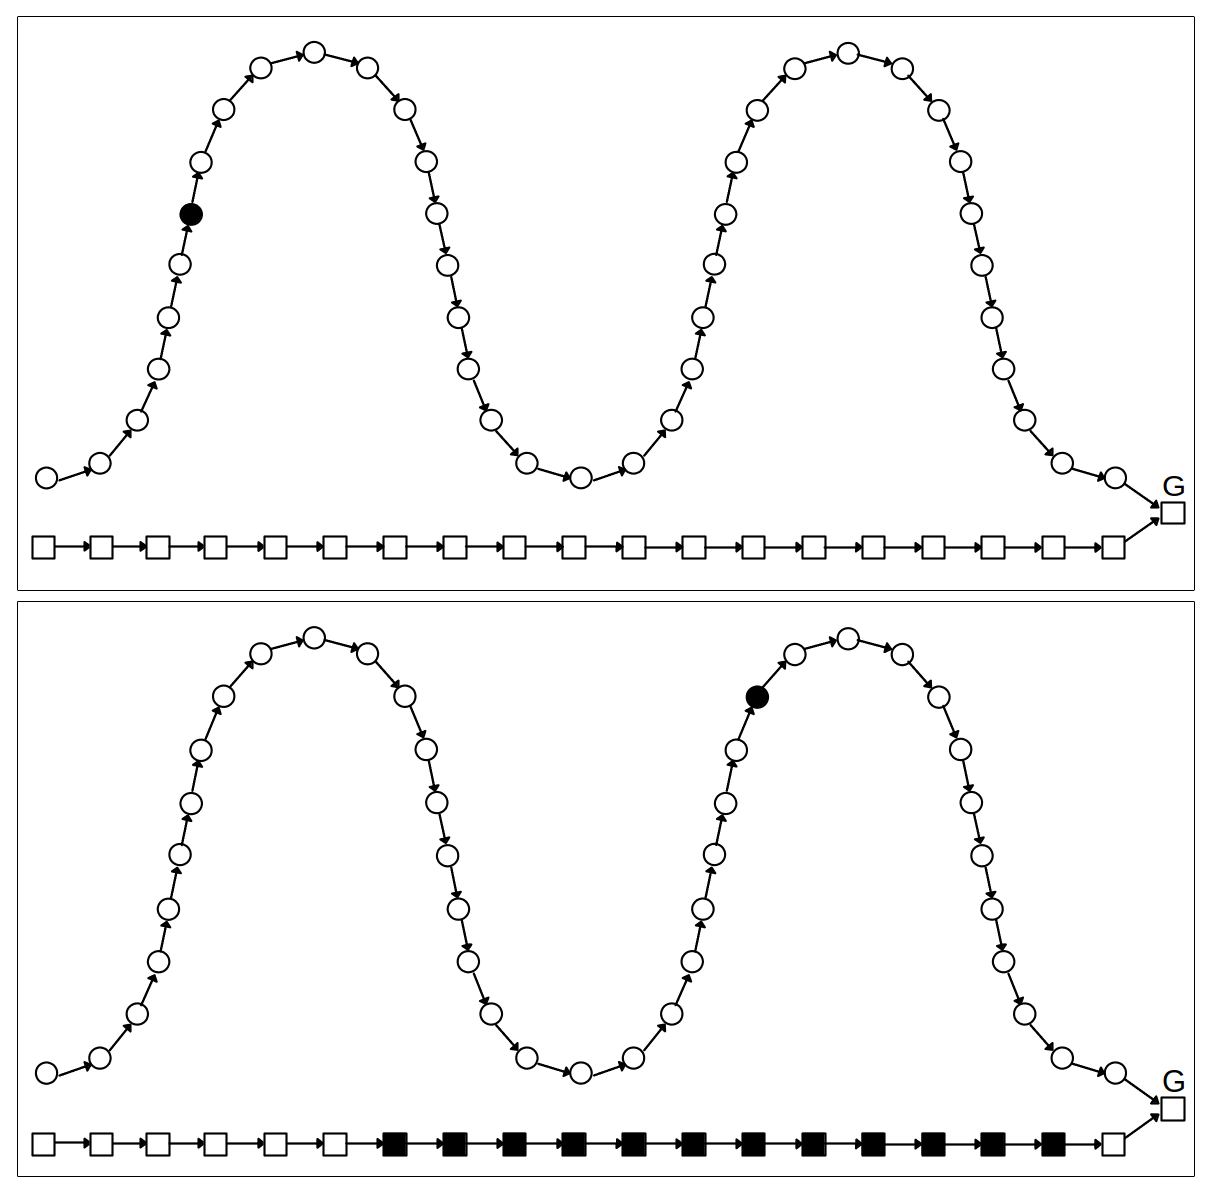
\includegraphics[width=8cm]{stim_E2a}
%\end{center}
%\caption{An example of an activation spreading over a network of Experiment 2. Here a continuous sequence of changes links R1 and I2 -- in other words this is the sequence of activations initiated by the chronologically first root change (curved branch) that eventually leads to the activation of the last immediate change and therefore G.} 
%\label{fig:3}
%\end{figure}


\textbf{Results}.  Network orientation (left or right) and position of the curved branch (top or bottom) had no effect and we collapsed across these variables.  Figure~\ref{fig:expt2}c summarizes the results for the three orders listed in Figures \ref{fig:expt2}a and \ref{fig:expt2}b. Consistent with Experiment 1,  \ev{R}{C} is preferred over \ev{R}{D} given the order \{\ev{R}{D},\ev{I}{D},\ev{R}{C},\ev{I}{C}\}, and a similar (but weaker) effect was found for the \{\ev{R}{D},\ev{R}{C},\ev{I}{D},\ev{I}{C}\} sequences. The critical finding is that \ev{R}{C} is also preferred for the \{\ev{R}{C},\ev{R}{D},\ev{I}{D},\ev{I}{C}\} sequences, even though the probability raising account makes the opposite prediction. STATISTICS HERE.

Relative to Experiment 1, the frequency with which \ev{I}{C} is chosen has increased in Experiment 2. This difference may reflect the increased difficulty of Experiment 2. When both branches of a dual branch structure are simultaneously active, keeping track of both root causes and the order in which they occurred is relatively challenging, which may lead some participants to fall back on the simple strategy fo choosing the immediate cause that directly precedes the effect.

%First we observed no significant effect (statistics?) of neither the orientation of the networks (left \textit{vs} right) nor the location of the curved chain (top \textit{vs} bottom). On average participants took 8 min to complete the experiment and overall 91\% of the time participants run an animation only once. Second the reversed response pattern for R1 and R2 between ``R1 cont'', ``R2 cont'' and ``State'' stimuli type shown in (Fig.\ref{fig:4}) confirms our hypothesis: when this is the first root change R1 that initiates a continuous sequence of changes until the activation of G, R1 is considered the cause of the activation of G about two times more than R2 (31\% against 15\%) while this is the opposite when this is the second root change that initiates a continuous sequence of changes (18\% against 29\%). Coherently, for ``State'' condition (when this is R2 that initiates the continuous sequence of changes) participants prefer R2 over R1 in a very large extent (47\% against 5\%). As expected the type of network had however no effect on the responses for I1 nor I2 and the percentages of responses for I2 and the root change that initiates the continuous sequence for the Event network (31\% and 34\% for respectively the ``R1 cont'' and ``R2 cont'' networks) were approximately the same.

\begin{figure}
\begin{center}
%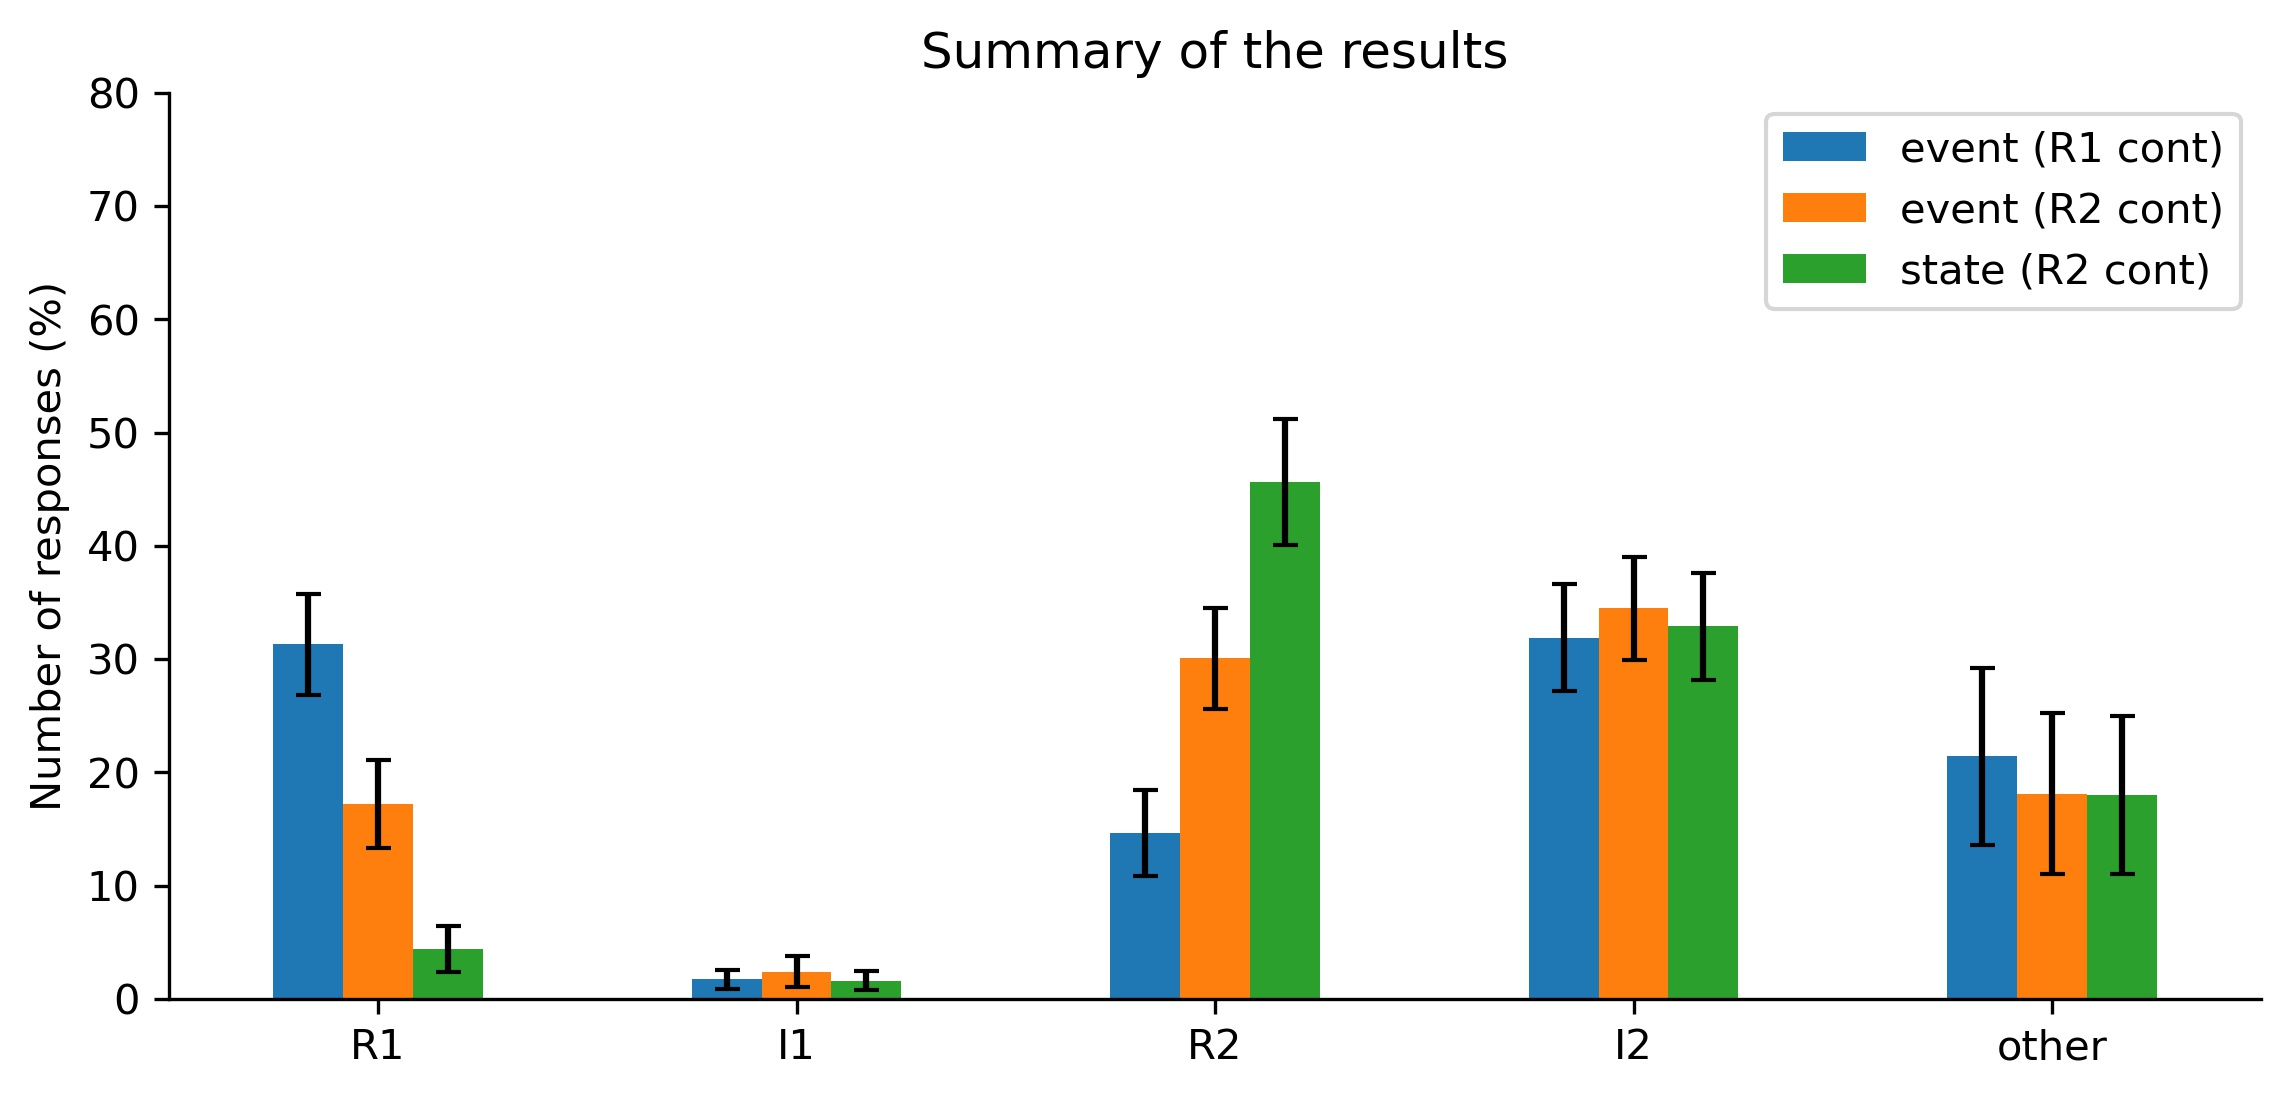
\includegraphics[width=8cm]{results_E2}
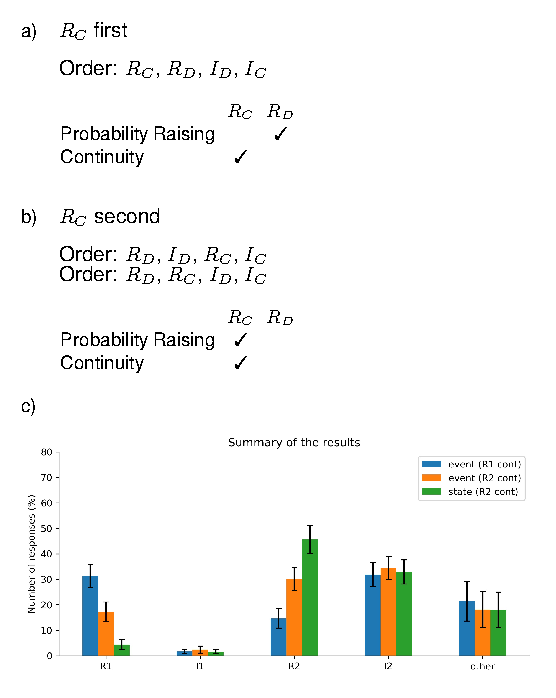
\includegraphics{figures/expt2.eps}
\end{center}
\caption{Experiment 2. (a) The probability raising and continuity accounts make different predictions for dual branch sequences in which \ev{R}{C} occurs before \ev{R}{D}. (b) The two accounts agree when \ev{R}{C} occurs after \ev{R}{D}.
(c) Responses for the three possible orders of the key events.} 
\label{fig:expt2}
\end{figure}

\section{General discussion}

Outline:

\textbf{I}. Summary and implications of the results

\textbf{II}. To say why these results cannot really be explained by the current theories of causation and why our theory can better account for them. I don't know if I should talk more about CF and PP accounts than I do in introduction, like saying something like that is probably not useful:

[\textit{According to the CF account, the general idea is that an event A is said to be a cause of a distinct event B if the occurrence of A makes a difference in the occurrence of B. More precisely A is a cause of B if and only if A and B are true, and A hadn't occurred B wouldn't have occurred. This interpretation calls upon counterfactual scenario or possible worlds where the presumed cause of the effect is removed from the system while all other relevant factors are kept as unchanged as possible compared to the actual world. According to us the main problem of this interpretation is that its best models explicitely rejects the idea of grounding causation on temporal information.
According to the PP account, an event A causes B when there is a physical connection between them. In one of its latest and probably most convincing formulation, this theory distinguishes two things : causal process and causal interaction (i.e. causation). A causal process is a physical process involving an object which conserves a certain quantity, like mass-energy, accross space and time. A causal interaction or causation is an exchange of that conserved quantity. However the theory goes sometimes against some of our best causal intuitions and to makes implicitely use of the CF analysis to explain our judgements: if I hold the head of my ennemy under water and make him die, I'm not genuinely the cause of his death; rather I'm actually preventing the possibility of a genuine causation which is breathing oxygen in order to live.}]

Or if I do have to explicit both theories I should insist on what the predictions of both theories are for our experiments and why they cannot explain people's intuition (the role of time).

\textbf{III}. To insist, maybe, on the work of Glymour where our project in part originated: explaining his caveat about treating events as pure propositions. To explain how our experiments extend this idea and insist more on the role of changes in continuous time. Maybe we should present some insights about how we could formalize further the model? How we could use formal tools like Graphical models?

\textbf{IV}. To present further experiments that would be interesting to make (with loops, cases of prevention, etc.)


\nocite{halpernp01}

\bibliographystyle{apacite}

\setlength{\bibleftmargin}{.125in}
\setlength{\bibindent}{-\bibleftmargin}

\bibliography{uber}


\end{document}
